% Figure s04f06_quasihole (Session 4): the Laughlin quasihole, its charge and its statistics.
% The image is rendered by figures/blender/s04f06_quasihole.py; the coordinates of the labels come from
% figures/blender/out/s04f06_quasihole_anchors.tex. Build with figures/blender/build_figure.sh s04f06_quasihole.
\documentclass[11pt,tikz,border=0pt]{standalone}
\usepackage[T1]{fontenc}
\usepackage{amsmath,amssymb,graphicx,bm}
\usepackage{xcolor}
\usetikzlibrary{arrows.meta,calc}
% The three label colors of the figures, with the same values as in src/figures_preamble.tex.
\definecolor{aqmaccent}{RGB}{31,78,121}
\definecolor{aqmbroken}{RGB}{168,42,34}
\definecolor{aqmmuted}{RGB}{125,125,125}

\newlength{\figw}\setlength{\figw}{16.51cm}   % 1.06 of the text width, before the empty margins of the render are cropped

\begin{document}
\begin{tikzpicture}[lbl/.style={font=\small, inner sep=1.5pt}, pnl/.style={font=\small\bfseries, inner sep=1.5pt}]
  \node[overlay, anchor=south west, inner sep=0pt] at (0,0)
    {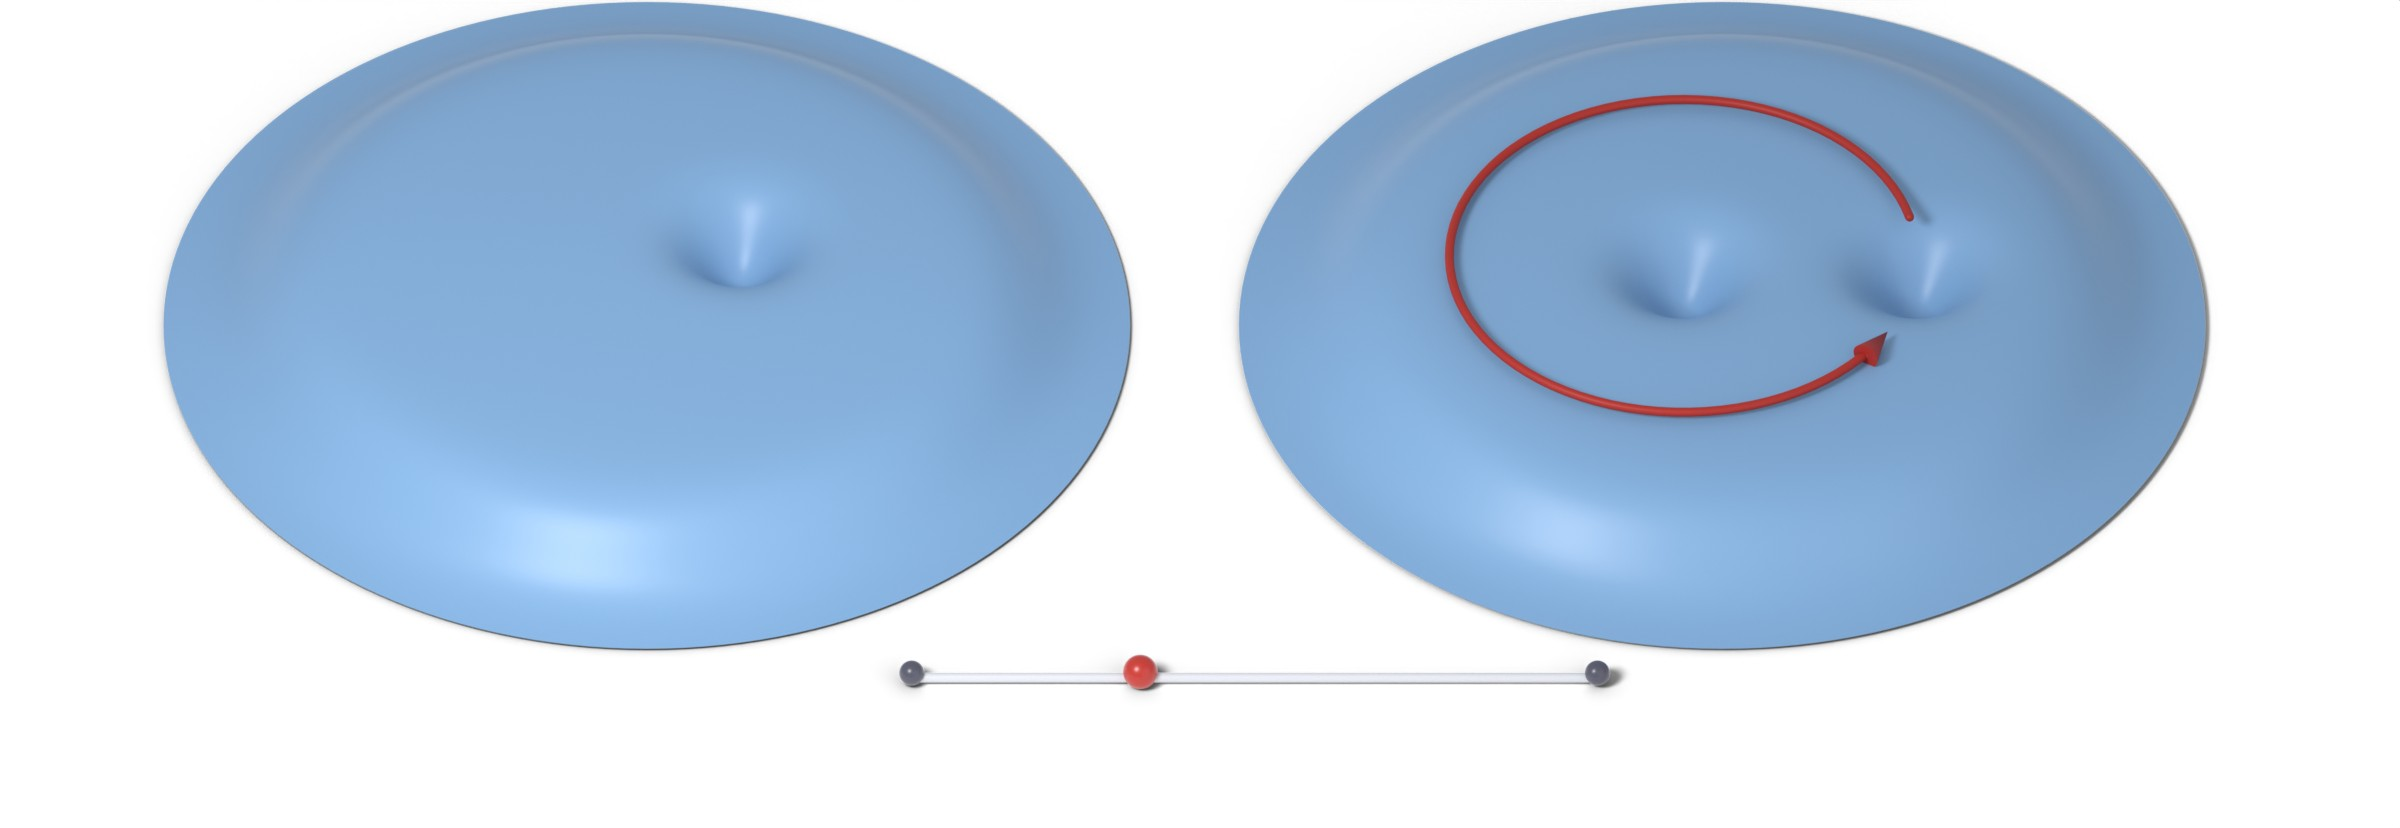
\includegraphics[width=\figw]{../blender/out/s04f06_quasihole.jpg}};
  % written by build_figure.sh; the painted part of the image
\path (0.0654\figw,0.0542\figw) rectangle (0.9217\figw,0.3438\figw);

  %% written by figlib.py; x and y in units of the image width
\coordinate (w) at (0.3084\figw,0.2220\figw);
\coordinate (apanel) at (0.0942\figw,0.3528\figw);
\coordinate (h1) at (0.7013\figw,0.2104\figw);
\coordinate (loop) at (0.7013\figw,0.3089\figw);
\coordinate (bpanel) at (0.5422\figw,0.3528\figw);
\coordinate (boson) at (0.3799\figw,0.0494\figw);
\coordinate (fermion) at (0.6656\figw,0.0494\figw);
\coordinate (anyon) at (0.4751\figw,0.0494\figw);
\coordinate (barlab) at (0.3636\figw,0.0627\figw);

  \node[pnl, anchor=south west] at (apanel) {(a)};
  \node[pnl, anchor=south west] at (bpanel) {(b)};
  \node[lbl, anchor=south west, align=left] at (w) {$w$, a charge\\$e/m$ missing};
  \node[lbl, anchor=south, text=aqmbroken, align=center] at (loop) {Aharonov-Bohm part $+\;2\pi/m$};
  \node[lbl, anchor=east] at (barlab) {exchange phase};
  \node[lbl, anchor=north] at (boson) {$0$, bosons};
  \node[lbl, anchor=north] at (fermion) {$\pi$, fermions};
  \node[lbl, anchor=north, text=aqmbroken] at (anyon) {$\pi/3$};
\end{tikzpicture}
\end{document}
